\documentclass[aspectratio=169,11pt]{beamer}
\usetheme{Madrid}
\usepackage[T1]{fontenc}
\usepackage{lmodern}
\usepackage{amsmath,amssymb}
\usepackage{booktabs,tabularx,multicol}
\usepackage{tikz}
\usetikzlibrary{arrows.meta,positioning,shapes.geometric,fit,calc}

% ---------- colours ----------
\definecolor{navy}{HTML}{1F3A5F}
\definecolor{accent}{HTML}{2A78D6}
\definecolor{warm}{HTML}{EB6834}
\definecolor{aqua}{HTML}{1BAF7A}
\definecolor{gold}{HTML}{EDA100}
\definecolor{soft}{HTML}{EEF3FA}
\definecolor{ink}{HTML}{333333}
\setbeamercolor{structure}{fg=navy}
\setbeamercolor{palette primary}{bg=navy,fg=white}
\setbeamercolor{palette secondary}{bg=navy!85!black,fg=white}
\setbeamercolor{palette tertiary}{bg=navy!70!black,fg=white}
\setbeamercolor{frametitle}{bg=navy,fg=white}
\setbeamercolor{title}{bg=navy,fg=white}
\setbeamercolor{block title}{bg=accent,fg=white}
\setbeamercolor{block body}{bg=soft,fg=ink}
\setbeamercolor{block title alerted}{bg=warm,fg=white}
\setbeamercolor{block body alerted}{bg=warm!8,fg=ink}
\setbeamercolor{block title example}{bg=aqua,fg=white}
\setbeamercolor{block body example}{bg=aqua!8,fg=ink}
\setbeamertemplate{navigation symbols}{}
\setbeamertemplate{itemize items}[circle]
\setbeamertemplate{section in toc}[sections numbered]

\newcommand{\code}[1]{\texttt{\small #1}}
\tikzset{
  box/.style={draw=navy,rounded corners=3pt,fill=soft,align=center,font=\scriptsize,minimum height=7mm,inner sep=3pt},
  hot/.style={box,fill=accent!15},
  arr/.style={-{Stealth[length=2mm]},thick,navy},
}
% attention-mask grid: #1 = name, #2 = test (\i row, \j col) returning allowed
\newcommand{\maskgrid}[3]{%
  \begin{tikzpicture}[scale=0.28]
    \foreach \i in {0,...,7}{\foreach \j in {0,...,7}{
      \pgfmathtruncatemacro{\ok}{#2}
      \ifnum\ok=1 \fill[accent] (\j,-\i) rectangle ++(0.92,-0.92);
      \else \fill[black!8] (\j,-\i) rectangle ++(0.92,-0.92); \fi }}
    \node[font=\scriptsize,anchor=north] at (4,-8.3) {#1};
    \node[font=\tiny,anchor=south] at (4,0.2) {#3};
  \end{tikzpicture}}

\title[CS-781 Capstone: Phase 1]{In-House Legal Intelligence System}
\subtitle{CS-781 Capstone: what the project is, and how Phase 1 is built}
\author[Manish Kumar]{Manish Kumar (251330604)}
\institute{CS-781, IIT Kanpur}
\date{Phase 1: 23 September -- 6 October 2026}

\begin{document}

\begin{frame}
  \titlepage
\end{frame}

\begin{frame}{Outline}
  \begin{multicols}{2}
  \tableofcontents
  \end{multicols}
\end{frame}

% =====================================================================
\section{The capstone}

\begin{frame}{The brief: a law firm that cannot use cloud LLMs}
  \begin{columns}[T]
    \begin{column}{0.55\textwidth}
      \begin{itemize}
        \item You are the new in-house AI developer at a law firm.
        \item Client matters and privileged material \alert{cannot leave the firm's infrastructure}.
              Sending them to a third-party LLM API is ruled out.
        \item The partners want a \textbf{self-hosted legal language foundation}.
              It must run entirely on hardware they control.
        \item It must then support the legal NLP tasks the firm needs every day.
        \item A rival engineer builds against the same brief, data and rules.
              The competition runs on a public Codabench leaderboard.
      \end{itemize}
    \end{column}
    \begin{column}{0.42\textwidth}
      \begin{block}{What ``success'' means}
        \begin{itemize}\small
          \item Not one lucky high score.
          \item A system you understand well enough to \textbf{defend, extend and fix}.
          \item Honest experiments: what worked, what failed, and why.
          \item Defended in a viva, as you would defend it to a sceptical partner.
        \end{itemize}
      \end{block}
    \end{column}
  \end{columns}
\end{frame}

\begin{frame}{Capstone at a glance: seven phases, one foundation model}
  \small
  \begin{tabularx}{\textwidth}{@{}clXXl@{}}
    \toprule
    \# & Task & Input & Output & Primary metric\\
    \midrule
    1 & Legal LM pre-training & 512-word legal prompt & 128-word continuation & BERTScore F1\\
    2 & Legal NER (L-NER) & legal document & character spans + labels & strict Macro-F1\\
    3 & Rhetorical Role (RR) & document sentences & one role per sentence & Macro-F1\\
    4 & Judgment Prediction (CJPE) & case text & binary 0/1 & Macro-F1\\
    5 & Statute Identification (LSI) & legal document & one or more statute IDs & Macro-F1\\
    6 & Abstractive Summarisation & legal document & generated summary & BERTScore F1\\
    7 & Prior Case Retrieval (PCR) & query + candidate pool & top-7 ranked IDs & Micro-F1@7\\
    8 & TBA (e.g.\ QA on your model) & TBA & TBA & TBA\\
    \bottomrule
  \end{tabularx}
  \vspace{2mm}
  \begin{center}
  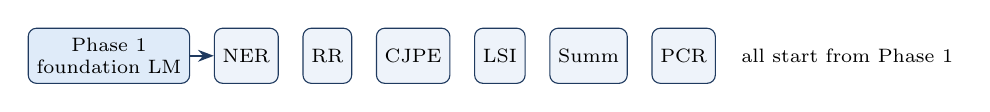
\begin{tikzpicture}[node distance=3mm]
    \node[hot] (p1) {Phase 1\\foundation LM};
    \foreach \n/\t [count=\k] in {p2/NER,p3/RR,p4/CJPE,p5/LSI,p6/Summ,p7/PCR}{
      \node[box,right=of p\the\numexpr\k\relax] (\n) {\t};}
    \draw[arr] (p1) -- (p2);
    \node[font=\scriptsize,right=2mm of p7] {all start from Phase 1};
  \end{tikzpicture}
  \end{center}
\end{frame}

\begin{frame}{Timeline (IST)}
  \begin{columns}[T]
    \begin{column}{0.5\textwidth}
      \small
      \begin{tabular}{@{}ll@{}}
        \toprule
        Milestone & Dates (2026)\\
        \midrule
        Codabench registration & 26 Sep, 12 noon\\
        \textbf{Phase 1: LM pre-training} & \textbf{23 Sep -- 6 Oct}\\
        Phase 2: L-NER & 7 -- 11 Oct\\
        Phase 3: RR & 12 -- 16 Oct\\
        Phase 4: CJPE & 17 -- 21 Oct\\
        Phase 5: LSI & 22 -- 26 Oct\\
        Phase 6: Summarisation & 27 Oct -- 2 Nov\\
        Phase 7: PCR & 3 -- 7 Nov\\
        Report + code & 8 Nov\\
        Viva & 9 -- 13 Nov (tentative)\\
        \bottomrule
      \end{tabular}
    \end{column}
    \begin{column}{0.46\textwidth}
      \begin{alertblock}{Deadlines are strict}
        \small
        Codabench needs 15--30 minutes per submission, and longer under load.
        Submit early in each window. Delay excuses are not accepted.
      \end{alertblock}
      \begin{block}{Submission counts}
        \small
        \begin{itemize}
          \item Phase 1: \textbf{at least 4}. Phases 2--7: \textbf{at least 6}.
          \item Max 40 per phase and 10 per day.
          \item Identical re-submissions do not count.
        \end{itemize}
      \end{block}
    \end{column}
  \end{columns}
\end{frame}

\begin{frame}{Data, access and the submission format}
  \begin{columns}[T]
    \begin{column}{0.5\textwidth}
      \begin{block}{Dataset}
        \small
        \code{Exploration-Lab/CS-781-Capstone} on Hugging Face (gated: accept the terms, then log in).
        There is one folder per phase, \code{Phase\_1\_Pretraining} to \code{Phase\_7\_PCR}.
        Test references are private.
      \end{block}
      \begin{alertblock}{Only official data}
        \small
        No external legal corpora, extra judgments, statutes or scraped court data.
      \end{alertblock}
    \end{column}
    \begin{column}{0.46\textwidth}
      \begin{block}{Same packaging in every phase}
        \small
        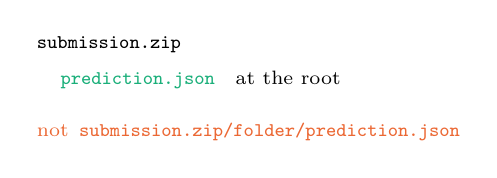
\begin{tikzpicture}[font=\ttfamily\scriptsize]
          \node[anchor=west] at (0,0) {submission.zip};
          \node[anchor=west] at (0.3,-0.45) {\textcolor{aqua}{\textbf{prediction.json}}\ \ \textrm{at the root}};
          \node[anchor=west] at (0,-1.1) {\textcolor{warm}{\textrm{not} submission.zip/folder/prediction.json}};
        \end{tikzpicture}
        \begin{itemize}
          \item Include \textbf{every} official test ID.
          \item Add \textbf{no} unknown ID. The evaluator checks both.
        \end{itemize}
      \end{block}
    \end{column}
  \end{columns}
\end{frame}

\begin{frame}{Phases 2--7: shared rules for adaptation}
  \begin{columns}[T]
    \begin{column}{0.52\textwidth}
      \begin{itemize}
        \item Start from \textbf{your own Phase-1 models}. Other pretrained models and LLM APIs are prohibited.
        \item Experiment with \textbf{all four} Phase-1 architectures. Fine-tuning a single model is not enough.
        \item At least \textbf{6 substantially different} experiments per phase:
          \begin{itemize}
            \item $\ge 5$ fine-tuning / PEFT techniques, and \alert{LORMA is compulsory};
            \item $\ge 1$ \alert{knowledge distillation} (teacher $\to$ smaller student).
          \end{itemize}
        \item Changing only hyperparameters does \textbf{not} make a new experiment.
      \end{itemize}
    \end{column}
    \begin{column}{0.44\textwidth}
      \begin{block}{Technique menu (varies by phase)}
        \small
        Full and partial fine-tuning, layer freezing, LoRA, QLoRA, AdaLoRA, rsLoRA,
        \textbf{LORMA}, Prefix tuning, Prompt tuning, Houlsby/Pfeiffer adapters,
        BitFit, IA$^3$, knowledge distillation.
      \end{block}
      \begin{exampleblock}{Why Phase 1 matters so much}
        \small
        All four Phase-1 models are reused six more times.
        Their tokenizer, context length and architecture shape every later phase.
      \end{exampleblock}
    \end{column}
  \end{columns}
\end{frame}

\begin{frame}{Phases 2 and 3: extraction and document structure}
  \begin{columns}[T]
    \begin{column}{0.49\textwidth}
      \begin{block}{Phase 2: Legal NER}
        \small
        \begin{itemize}
          \item Output \code{[start, end, label]} character spans per document.
          \item 12 labels: APP, RESP, A.COUNSEL, R.COUNSEL, JUDGE, WIT, AUTH, COURT, STAT, PREC, DATE, CASENO.
          \item \textbf{Strict} matching. An offset that is off by one character counts as wrong.
          \item Key issues: character-to-token alignment, boundary errors, boilerplate false positives, class imbalance.
        \end{itemize}
      \end{block}
    \end{column}
    \begin{column}{0.49\textwidth}
      \begin{block}{Phase 3: Rhetorical roles}
        \small
        \begin{itemize}
          \item Output exactly one label per sentence, in order.
          \item 13 labels, e.g.\ Fact, Issue, ArgumentPetitioner, Statute, PrecedentReliedUpon, RatioOfTheDecision, RulingByPresentCourt, None.
          \item Two domains: Corporate Law (CL) and IT.
          \item Key issues: sentence versus document context, and confusable roles.
        \end{itemize}
      \end{block}
    \end{column}
  \end{columns}
\end{frame}

\begin{frame}{Phases 4 and 5: decisions and statutes}
  \begin{columns}[T]
    \begin{column}{0.49\textwidth}
      \begin{block}{Phase 4: Court judgment prediction}
        \small
        \begin{itemize}
          \item Predict a binary outcome: \code{\{"id":..., "pred": 0|1\}}.
          \item Judgments are \textbf{long}. Options include chunking, sliding windows, hierarchical or attention pooling, and section selection.
          \item Scored by Macro-F1, so both classes matter. Handle class imbalance.
        \end{itemize}
      \end{block}
    \end{column}
    \begin{column}{0.49\textwidth}
      \begin{block}{Phase 5: Legal statute identification}
        \small
        \begin{itemize}
          \item \textbf{Multi-label}: output a set of statute IDs per document.
          \item Needs multi-label loss, class weights and rare-statute handling.
          \item \textbf{Thresholds} can be global or per label, with calibration.
          \item Macro-F1 rewards getting rare statutes right.
        \end{itemize}
      \end{block}
    \end{column}
  \end{columns}
\end{frame}

\begin{frame}{Phases 6 and 7: generation and retrieval}
  \begin{columns}[T]
    \begin{column}{0.49\textwidth}
      \begin{block}{Phase 6: Abstractive summarisation}
        \small
        \begin{itemize}
          \item Generate a concise summary of a long legal document.
          \item Scored by BERTScore F1, with ROUGE-1 and ROUGE-L as secondary metrics.
          \item Needs hierarchical or chunk-then-summarise strategies, length control and redundancy control.
          \item Phase-1 generation quality carries over directly.
        \end{itemize}
      \end{block}
    \end{column}
    \begin{column}{0.49\textwidth}
      \begin{block}{Phase 7: Prior case retrieval}
        \small
        \begin{itemize}
          \item Rank 7 unique candidate IDs per query, taken from that split's candidate pool.
          \item Scored by Micro-F1@7 against the full gold set.
          \item Options include contrastive or pairwise objectives, hard negatives, pooling and chunked representations.
          \item The student model in distillation learns from teacher similarity scores.
        \end{itemize}
      \end{block}
    \end{column}
  \end{columns}
\end{frame}

\begin{frame}{How the project is graded, and the integrity rules}
  \begin{columns}[T]
    \begin{column}{0.48\textwidth}
      \begin{block}{Leaderboard is only one criterion}
        \small
        \begin{itemize}
          \item Data analysis and preprocessing
          \item Minimum submissions and real experimentation
          \item Code quality, documentation and the GitHub repository
          \item Analysis of what worked and failed, and why
          \item Novelty within the compute limits
          \item Private-test performance and rank
          \item Viva performance and report quality
        \end{itemize}
      \end{block}
    \end{column}
    \begin{column}{0.48\textwidth}
      \begin{alertblock}{Rules}
        \small
        \begin{itemize}
          \item Individual work. Similar submissions can lead to an \textbf{F grade}.
          \item LLMs \textbf{may} help with ancillary code (plots) and with understanding architectures.
          \item LLMs \textbf{may not} write the model architecture, tune hyperparameters, or analyse results.
          \item The LLM declaration is mandatory. Cite every paper and snippet used.
          \item Compute budget: free Colab or Kaggle GPUs. Checkpoint often.
        \end{itemize}
      \end{alertblock}
    \end{column}
  \end{columns}
\end{frame}

\begin{frame}[fragile]{Final deliverables}
  \begin{columns}[T]
    \begin{column}{0.5\textwidth}
      \small
\begin{verbatim}
CS781-CP-First-Last-Roll-report_code.zip
|-- code/
|   |-- phase1/
|   |-- phase2/  ...
`-- report/
    `-- CS781-CP-...-report.pdf
\end{verbatim}
      \vspace{-2mm}
      \begin{itemize}
        \item No extra wrapper folder.
        \item Submitted on Hello IITK.
        \item Include a GitHub repository with a detailed README for each phase and submission.
      \end{itemize}
    \end{column}
    \begin{column}{0.46\textwidth}
      \begin{block}{The report (LaTeX) must explain}
        \small
        \begin{enumerate}
          \item the problem and the data used;
          \item the baselines tried and the final approach;
          \item the experiments that led there;
          \item what failed and why;
          \item what the results show, the remaining limitations, and the next steps.
        \end{enumerate}
        It should be reasoning, not a gallery of leaderboard screenshots.
      \end{block}
    \end{column}
  \end{columns}
\end{frame}

% =====================================================================
\section{Phase 1: the task}

\begin{frame}[fragile]{Phase 1: continue legal text}
  \begin{columns}[T]
    \begin{column}{0.48\textwidth}
      \textbf{Input:} a 512-word legal prompt.
      \scriptsize
\begin{verbatim}
{ "1": {"text": "The issue involved in
         these petitions is ..."},
  "2": {"text": "In ..."} }
\end{verbatim}
      \normalsize\textbf{Output:} a 128-word continuation for each ID.\scriptsize
\begin{verbatim}
{ "1": {"text": "<128 generated words>"},
  "2": {"text": "..."} }
\end{verbatim}
      \small The output must contain \alert{only the continuation}, never the prompt.
    \end{column}
    \begin{column}{0.48\textwidth}
      \begin{block}{Metrics}
        \small
        \begin{itemize}
          \item \textbf{Primary:} BERTScore F1, which measures semantic similarity to the hidden true continuation.
          \item \textbf{Secondary:} ROUGE-L F1 (longest common subsequence) and BLEU-4 (n-gram precision).
        \end{itemize}
      \end{block}
      \begin{exampleblock}{The model is the real product}
        \small
        The Phase-1 model is the \textbf{foundation} for Phases 2--7.
        Its tokenizer, context length and quality are inherited everywhere.
      \end{exampleblock}
    \end{column}
  \end{columns}
\end{frame}

\begin{frame}{Phase 1 rules}
  \begin{columns}[T]
    \begin{column}{0.48\textwidth}
      \begin{block}{Must}
        \small
        \begin{itemize}
          \item Train \textbf{from scratch} on the provided corpus.
          \item Stay within \textbf{50M -- 300M parameters}.
          \item Implement and train your own architecture.
          \item Stay practical on free Colab or Kaggle GPUs.
          \item Explore \textbf{at least four substantially different architectures}.
        \end{itemize}
      \end{block}
      \begin{exampleblock}{Allowed}
        \small
        The course BPE tokenizer or a new tokenizer, static embeddings (Word2Vec, GloVe), and any amount of the provided corpus.
      \end{exampleblock}
    \end{column}
    \begin{column}{0.48\textwidth}
      \begin{alertblock}{Not allowed}
        \small
        \begin{itemize}
          \item Pretrained language models or pretrained weights (HF, fairseq, \ldots).
          \item External legal corpora or datasets.
          \item Closed commercial APIs for training, inference or evaluation.
          \item Any foundation model above 300M parameters.
        \end{itemize}
      \end{alertblock}
      \begin{block}{Different means different}
        \small
        Changing width, depth, heads or learning rate of the \emph{same} design does \textbf{not} count as a new architecture.
      \end{block}
    \end{column}
  \end{columns}
\end{frame}

\begin{frame}{Phase 1 data}
  \begin{columns}[T]
    \begin{column}{0.52\textwidth}
      \small
      \begin{tabular}{@{}lr@{}}
        \toprule
        File (\code{Phase\_1\_Pretraining/}) & Size\\
        \midrule
        \code{Train/train\_acts.json} & 0.73 GB\\
        \code{Train/train\_supreme\_court.json} & 1.32 GB\\
        \code{Train/train\_tribunals.json} & 6.48 GB\\
        \code{Train/train\_high\_courts.json} & 10.67 GB\\
        \code{Test/test.json} & 3 MB\\
        \bottomrule
      \end{tabular}
      \vspace{2mm}
      \begin{itemize}
        \item More than \textbf{4.5 billion tokens} in total.
        \item No development split is provided. \alert{You build your own.}
        \item The starter notebook uses about 200M training and 5M validation tokens, a GPT-2 tokenizer, a 2048 context, and 8 layers $\times$ 8 heads $\times$ 560 dimensions.
      \end{itemize}
    \end{column}
    \begin{column}{0.44\textwidth}
      \begin{block}{Consequences for the design}
        \small
        \begin{itemize}
          \item The files cannot be loaded into RAM, so they must be \textbf{streamed}.
          \item Compute, not data, is the limit. Choosing \emph{which} tokens to use is an experiment in itself.
          \item The four sources differ in style. Acts are statutory text; the others are judgments.
          \item The test prompts cannot be scored locally, so we build a \textbf{dev set} in the same format.
        \end{itemize}
      \end{block}
    \end{column}
  \end{columns}
\end{frame}

\begin{frame}{What the experiments should cover}
  \small
  \begin{columns}[T]
    \begin{column}{0.49\textwidth}
      \begin{itemize}
        \item \textbf{Tokenizer:} BPE versus others, vocabulary size, tokens per word.
        \item \textbf{Data mixing:} which sources, and in what ratios.
        \item \textbf{Architecture:} attention, feed-forward, normalisation and positional scheme.
        \item \textbf{Context length:} long-range legal dependencies versus compute.
        \item \textbf{Training:} learning-rate schedule, warm-up, batch size, accumulation and duration.
      \end{itemize}
    \end{column}
    \begin{column}{0.49\textwidth}
      \begin{itemize}
        \item \textbf{Regularisation:} dropout and weight decay.
        \item \textbf{Validation:} split construction, early stopping and checkpoint choice.
        \item \textbf{Decoding:} temperature, top-$k$, top-$p$ and repetition control.
        \item \textbf{Compression:} knowledge distillation into a compact model.
        \item \textbf{Key question:} how does validation perplexity relate to generation quality?
      \end{itemize}
    \end{column}
  \end{columns}
  \vspace{3mm}
  \begin{exampleblock}{}
    \centering ``A weaker model with clear evidence and thoughtful analysis is more valuable than an unexplained lucky submission.''
  \end{exampleblock}
\end{frame}

% =====================================================================
\section{Phase 1: our pipeline}

\begin{frame}{End-to-end pipeline: seven small scripts}
  \centering
  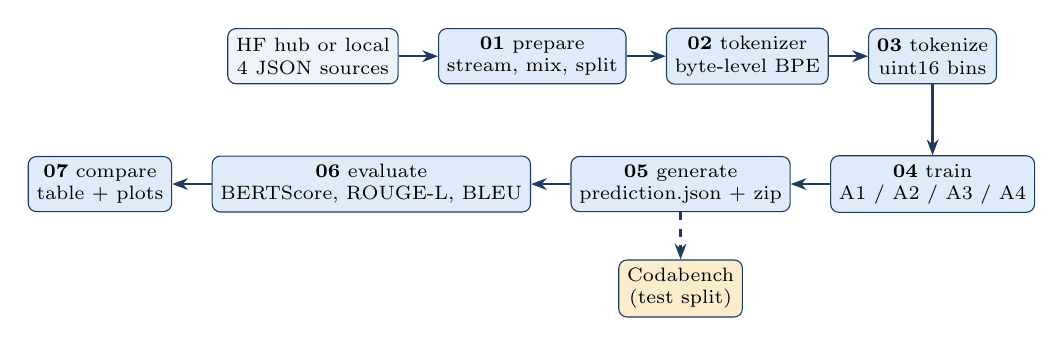
\begin{tikzpicture}[node distance=4mm and 5mm]
    \node[box] (hf) {HF hub or local\\4 JSON sources};
    \node[hot,right=of hf] (s1) {\textbf{01} prepare\\stream, mix, split};
    \node[hot,right=of s1] (s2) {\textbf{02} tokenizer\\byte-level BPE};
    \node[hot,right=of s2] (s3) {\textbf{03} tokenize\\uint16 bins};
    \node[hot,below=9mm of s3] (s4) {\textbf{04} train\\A1 / A2 / A3 / A4};
    \node[hot,left=of s4] (s5) {\textbf{05} generate\\prediction.json + zip};
    \node[hot,left=of s5] (s6) {\textbf{06} evaluate\\BERTScore, ROUGE-L, BLEU};
    \node[hot,left=of s6] (s7) {\textbf{07} compare\\table + plots};
    \draw[arr] (hf) -- (s1); \draw[arr] (s1) -- (s2); \draw[arr] (s2) -- (s3);
    \draw[arr] (s3) -- (s4); \draw[arr] (s4) -- (s5); \draw[arr] (s5) -- (s6); \draw[arr] (s6) -- (s7);
    \node[box,below=6mm of s5,fill=gold!20] (cb) {Codabench\\(test split)};
    \draw[arr,dashed] (s5) -- (cb);
  \end{tikzpicture}
  \vspace{3mm}
  \begin{itemize}\small
    \item One YAML file per architecture \emph{inherits} \code{base.yaml}. All four share data, tokenizer, budget and schedule, which makes the comparison \textbf{controlled}.
    \item Any value can be changed from the command line, e.g.\ \code{--set train.lr=3e-4 run\_name=A1\_lr3e-4}.
    \item Every run saves its resolved config, a metrics log, a summary, and best and last checkpoints.
  \end{itemize}
\end{frame}

\begin{frame}{Step 01: streaming, mixing and splitting}
  \begin{columns}[T]
    \begin{column}{0.5\textwidth}
      \small
      \begin{itemize}
        \item Files are read \textbf{record by record} with \code{ijson}, over HTTP from the hub.
              Nothing is fully downloaded.
        \item The JSON layout is auto-detected: array, JSON Lines, or ID-keyed object.
        \item Source $s$ with ratio $r_s$ receives a budget of $B\cdot r_s$ tokens.
              The default is $B=200$M with Acts 0.10, SC 0.30, HC 0.35 and Tribunals 0.25.
        \item Documents are skipped at random (\code{doc\_keep\_prob}) so reads spread across each file.
        \item The train/val split is made \textbf{by document}, so no validation text leaks into training.
      \end{itemize}
    \end{column}
    \begin{column}{0.46\textwidth}
      \begin{block}{Local dev set = a copy of the test format}
        \small
        From each held-out document we take a random window of 640 words:
        \[
          \underbrace{w_1\ldots w_{512}}_{\text{dev\_prompts.json}}\;
          \underbrace{w_{513}\ldots w_{640}}_{\text{dev\_references.json}}
        \]
        This lets us compute BERTScore, ROUGE-L and BLEU-4 locally before spending a Codabench submission.
      \end{block}
    \end{column}
  \end{columns}
\end{frame}

\begin{frame}{Step 02: a legal byte-level BPE tokenizer}
  \begin{columns}[T]
    \begin{column}{0.52\textwidth}
      \small
      \begin{itemize}
        \item BPE starts from the 256 bytes and \textbf{repeatedly merges the most frequent adjacent pair} until it reaches the target vocabulary size (default 32k).
        \item Byte-level means there are \textbf{no unknown tokens}: Devanagari names, ``\S'', and OCR noise can all be encoded.
        \item Trained on legal text, frequent words such as \emph{appellant}, \emph{respondent} and \emph{Section} become single tokens.
        \item Special tokens are \code{<|endoftext|>} for document boundaries and \code{<|pad|>}.
      \end{itemize}
    \end{column}
    \begin{column}{0.44\textwidth}
      \begin{block}{Efficiency metric: fertility}
        \small
        \[
          \text{fertility}=\frac{\#\text{tokens}}{\#\text{words}}
        \]
        Lower fertility means shorter sequences. More of the 512-word prompt then fits in the context, and training covers more text per step.
      \end{block}
      \begin{exampleblock}{Experiment}
        \small
        Compare legal BPE at 16k, 32k and 48k against GPT-2's 50k vocabulary.
        Measure tokens per word, validation loss, and the parameters spent on the embedding table.
      \end{exampleblock}
    \end{column}
  \end{columns}
\end{frame}

\begin{frame}{Step 03 and the language-modelling objective}
  \begin{columns}[T]
    \begin{column}{0.48\textwidth}
      \small
      \textbf{Token bins.} All documents are joined with \code{<|endoftext|>} into one flat \code{uint16} file.
      Training reads random windows through a memory map, so RAM use stays tiny.
      \vspace{2mm}

      \textbf{Causal LM.} For a sequence $x_1\ldots x_T$:
      \[
        \mathcal{L}=-\frac{1}{T}\sum_{t=1}^{T}\log p_\theta(x_t\mid x_{<t}),
        \qquad \text{PPL}=e^{\mathcal{L}}
      \]
    \end{column}
    \begin{column}{0.48\textwidth}
      \begin{block}{Continuation loss: one metric for all four models}
        \small
        With a prefix of length $p$ as context, score only the tokens after it:
        \[
          \mathcal{L}_{\text{cont}}=-\frac{1}{T-p}\sum_{t=p+1}^{T}\log p_\theta(x_t\mid x_{\le p},\,x_{p+1..t-1})
        \]
        Validation uses $p=768$ and scores the next 257 tokens for \emph{every} architecture.
        This mirrors the task of reading the prompt and then writing.
      \end{block}
    \end{column}
  \end{columns}
\end{frame}

\begin{frame}{One interface, four objectives: the \code{prefix\_len} trick}
  \small
  Every model implements \code{model(idx, p)}, returning logits that predict \code{idx[:, p:]}.
  \vspace{1mm}

  \begin{tabularx}{\textwidth}{@{}lXX@{}}
    \toprule
    Model & Training prefix length & What the prefix does\\
    \midrule
    A1 GPT & always 1, so every token is supervised & read causally\\
    A2 Enc--dec & random in $[L/4,\,L-64]$ & encoder reads it, decoder writes\\
    A3 Prefix-LM & 1 with probability 0.5, else random in $[64,\,0.75L]$ & read \textbf{bidirectionally} in the same stack\\
    A4 Efficient & always 1 & read causally (local + global)\\
    \bottomrule
  \end{tabularx}
  \vspace{1mm}
  \begin{columns}[T]
    \begin{column}{0.48\textwidth}
      \begin{block}{Why it helps}
        \small
        One trainer, evaluator and generation loop serve all four models.
      \end{block}
    \end{column}
    \begin{column}{0.48\textwidth}
      \begin{alertblock}{Trade-off to analyse}
        \small
        A2 and A3 do not score the prefix, so fewer tokens are supervised. Do they still win?
      \end{alertblock}
    \end{column}
  \end{columns}
\end{frame}

% =====================================================================
\section{Phase 1: the four architectures}

\begin{frame}{Attention masks: the core difference}
  \centering
  \maskgrid{A1 causal}{\j<=\i ? 1 : 0}{GPT (A1), decoder self-attn (A2)}\hspace{4mm}
  \maskgrid{A2 encoder}{1}{bidirectional over prompt}\hspace{4mm}
  \maskgrid{A3 prefix-LM ($p=4$)}{(\j<4 || \j<=\i) ? 1 : 0}{bidirectional prompt + causal rest}\hspace{4mm}
  \maskgrid{A4 local, $W=3$}{(\j<=\i && \j>\i-3) ? 1 : 0}{sliding window (some layers)}
  \vspace{3mm}

  \small
  Rows are queries and columns are keys. A blue cell means the query may attend to that key.
  A4 uses the local mask in most layers and the full causal mask in every third layer.
\end{frame}

\begin{frame}{A1: decoder-only Transformer (GPT-2 style), the baseline}
  \begin{columns}[T]
    \begin{column}{0.4\textwidth}
      \centering
      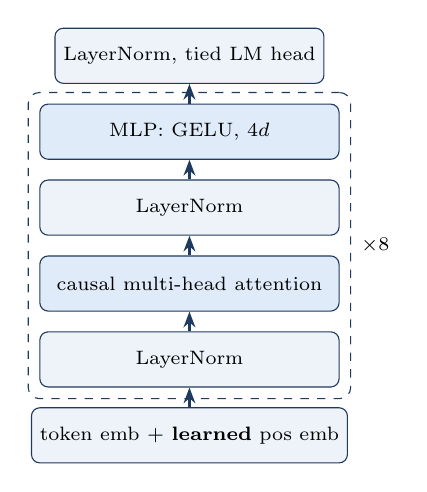
\begin{tikzpicture}[node distance=2.5mm]
        \node[box] (e) {token emb + \textbf{learned} pos emb};
        \node[box,above=of e,minimum width=38mm] (ln1) {LayerNorm};
        \node[hot,above=of ln1,minimum width=38mm] (att) {causal multi-head attention};
        \node[box,above=of att,minimum width=38mm] (ln2) {LayerNorm};
        \node[hot,above=of ln2,minimum width=38mm] (ff) {MLP: GELU, $4d$};
        \node[box,above=of ff] (h) {LayerNorm, tied LM head};
        \node[draw=navy,dashed,rounded corners,fit=(ln1)(ff),inner sep=4pt,label={[font=\scriptsize]right:$\times 8$}] {};
        \draw[arr] (e)--(ln1); \draw[arr](ln1)--(att); \draw[arr](att)--(ln2); \draw[arr](ln2)--(ff); \draw[arr](ff)--(h);
      \end{tikzpicture}
    \end{column}
    \begin{column}{0.56\textwidth}
      \small
      \begin{itemize}
        \item Pre-LN residual block: $x \leftarrow x + \text{Attn}(\text{LN}(x))$, then $x \leftarrow x + \text{MLP}(\text{LN}(x))$.
        \item Attention: $\text{softmax}\!\big(QK^\top/\sqrt{d_h} + M_{\text{causal}}\big)V$.
        \item Positions come from a learned table of 1024 rows, so the model \alert{cannot read beyond 1024 tokens}.
        \item The output head is tied to the embedding matrix, which saves $V\cdot d$ parameters.
        \item Uses $d=768$, 8 layers and 12 heads, for \textbf{82.1M} parameters.
      \end{itemize}
      \begin{block}{Role in the study}
        \small
        The reference point, closest to the starter notebook. Every other design is measured against it.
      \end{block}
    \end{column}
  \end{columns}
\end{frame}

\begin{frame}{A2: encoder--decoder Transformer}
  \begin{columns}[T]
    \begin{column}{0.48\textwidth}
      \centering
      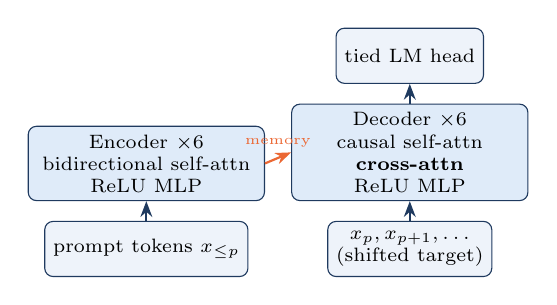
\begin{tikzpicture}[node distance=2.5mm]
        \node[box] (src) {prompt tokens $x_{\le p}$};
        \node[hot,above=of src,minimum width=30mm] (enc) {Encoder $\times 6$\\bidirectional self-attn\\ReLU MLP};
        \node[box,right=10mm of src] (tgt) {$x_p, x_{p+1},\ldots$\\(shifted target)};
        \node[hot,above=of tgt,minimum width=30mm] (dec) {Decoder $\times 6$\\causal self-attn\\\textbf{cross-attn}\\ReLU MLP};
        \node[box,above=of dec] (out) {tied LM head};
        \draw[arr](src)--(enc); \draw[arr](tgt)--(dec); \draw[arr](dec)--(out);
        \draw[arr,warm] (enc.east) -- node[above,font=\tiny]{memory} (dec.west);
      \end{tikzpicture}
    \end{column}
    \begin{column}{0.48\textwidth}
      \small
      \begin{itemize}
        \item Each block is cut at a random point $p$. The encoder reads $[0,p)$ and the decoder predicts $[p,L)$.
        \item The decoder input starts with the \emph{last prompt token}, so no BOS token is needed.
        \item Fixed \textbf{sinusoidal} positions, with embeddings scaled by $\sqrt{d}$ as in Vaswani et al.
        \item Uses $d=640$ and 6+6 layers, for \textbf{89.4M} parameters.
      \end{itemize}
      \begin{exampleblock}{Hypothesis}
        \small
        The objective matches the task: read the prompt, then write.
      \end{exampleblock}
    \end{column}
  \end{columns}
\end{frame}

\begin{frame}{A3: hybrid prefix-LM with ALiBi (UniLM / GLM style)}
  \begin{columns}[T]
    \begin{column}{0.5\textwidth}
      \small
      \begin{itemize}
        \item One stack is an encoder for the prompt and a decoder for the continuation. Only the mask changes, and there is no cross-attention.
        \item There are \textbf{no position embeddings}. ALiBi adds a distance penalty per head $h$:
        \[
          \text{score}_{ij} = \frac{q_i^\top k_j}{\sqrt{d_h}} - m_h\,|i-j|,\quad m_h = 2^{-8h/H}
        \]
        \item ALiBi can extrapolate to longer inputs than seen in training.
        \item Half the examples are plain causal; the rest use a random prefix. 8 layers, $d=768$, \textbf{81.3M} parameters.
      \end{itemize}
    \end{column}
    \begin{column}{0.46\textwidth}
      \centering
      \maskgrid{mask with $p=4$}{(\j<4 || \j<=\i) ? 1 : 0}{prompt $|$ continuation}
      \vspace{2mm}
      \begin{block}{Hypothesis}
        \small
        Bidirectional reading of the prompt gives a richer context representation than A1, without A2's extra encoder parameters.
      \end{block}
    \end{column}
  \end{columns}
\end{frame}

\begin{frame}{A4: efficient decoder (LLaMA, Mistral and Gemma-2 ideas)}
  \begin{columns}[T]
    \begin{column}{0.52\textwidth}
      \small
      \begin{itemize}
        \item \textbf{Grouped-query attention}: 12 query heads share 4 KV heads, so the KV-cache is $3\times$ smaller.
        \item \textbf{Sliding window} $W=256$ costs $O(TW)$, not $O(T^2)$. Every third layer is global.
        \item \textbf{RoPE} rotates $q$ and $k$ by angle $\theta_i\cdot\text{pos}$, so scores depend on relative position.
        \item \textbf{RMSNorm} $x/\sqrt{\tfrac1d\sum x_i^2+\epsilon}\odot g$ and \textbf{SwiGLU} $W_2\big(\text{SiLU}(W_g x)\odot W_u x\big)$, with no biases.
        \item 10 layers, $d=768$, \textbf{87.5M} parameters.
      \end{itemize}
    \end{column}
    \begin{column}{0.44\textwidth}
      \centering
      \maskgrid{local layer, $W=3$}{(\j<=\i && \j>\i-3) ? 1 : 0}{rolling cache of $W-1$ keys}
      \vspace{2mm}
      \begin{block}{Hypothesis}
        \small
        Better quality per FLOP. Faster generation, and a smaller memory footprint for long legal documents in Phases 4--7.
      \end{block}
    \end{column}
  \end{columns}
\end{frame}

\begin{frame}{The four designs side by side}
  \small
  \begin{tabularx}{\textwidth}{@{}l*{4}{>{\raggedright\arraybackslash}X}@{}}
    \toprule
     & \textbf{A1 GPT} & \textbf{A2 Enc--Dec} & \textbf{A3 Prefix-LM} & \textbf{A4 Efficient}\\
    \midrule
    Stacks & 1 decoder & encoder + decoder & 1 shared & 1 decoder\\
    Prompt attention & causal & bidirectional & bidirectional & causal, local/global\\
    Positions & learned absolute & sinusoidal & ALiBi (relative) & RoPE (relative)\\
    Norm & LayerNorm & LayerNorm & LayerNorm & RMSNorm\\
    MLP & GELU & ReLU & GELU & SwiGLU\\
    KV heads & 12 & 10 & 12 & \textbf{4} (GQA)\\
    Extra & -- & cross-attention & prefix mask & sliding window\\
    Objective & causal LM & prefix $\to$ continuation & mixed causal/prefix & causal LM\\
    Parameters & 82.1M & 89.4M & 81.3M & 87.5M\\
    \bottomrule
  \end{tabularx}
  \vspace{2mm}

  All four use the 32k legal BPE, a 1024-token context, and a tied output head.
  Parameter counts are matched to within 10\%, so differences come from \textbf{design}, not size.
\end{frame}

\begin{frame}{Where the parameters go}
  \begin{columns}[T]
    \begin{column}{0.5\textwidth}
      \small
      For a standard block with width $d$ and MLP width $4d$:
      \[
        \underbrace{4d^2}_{Q,K,V,O} + \underbrace{8d^2}_{\text{MLP}} = 12d^2
      \]
      For $d=768$ that is 7.1M per layer, or 56.6M for 8 layers.
      \vspace{1mm}

      The embedding table adds $V\cdot d = 32{,}064\times768 = 24.6$M.
      \vspace{1mm}

      Total: about \textbf{82M}, inside the 50--300M window.
    \end{column}
    \begin{column}{0.46\textwidth}
      \begin{block}{Levers the rules leave open}
        \small
        \begin{itemize}
          \item The vocabulary size trades embedding parameters against fertility.
          \item GQA and SwiGLU re-spend parameters: $d_{ff}=2048$ with 3 matrices costs about the same as a $4d$ GELU MLP.
          \item There is room to scale to 150--300M if the GPU time allows. Compare the gain against the extra time per step.
        \end{itemize}
      \end{block}
    \end{column}
  \end{columns}
\end{frame}

% =====================================================================
\section{Phase 1: training, decoding, evaluation}

\begin{frame}{Step 04: one training loop for every architecture}
  \begin{columns}[T]
    \begin{column}{0.52\textwidth}
      \small
      \begin{itemize}
        \item \textbf{AdamW} with $\beta=(0.9,0.95)$ and weight decay 0.1 on matrices only.
        \item \textbf{Linear warm-up then cosine decay}:
          \[
            \eta_t=\eta_{\min}+\tfrac12(\eta_{\max}-\eta_{\min})\big(1+\cos\pi\tfrac{t-t_w}{T-t_w}\big)
          \]
        \item Batch: $8\times 8$ accumulation $\times$ 1024 = 65k tokens per step. 3000 steps is about 197M tokens.
        \item \textbf{Mixed precision}: bf16, or fp16 with a GradScaler on a T4. Gradients are clipped at 1.0.
        \item Validation every 250 steps on fixed blocks; the best checkpoint is kept.
      \end{itemize}
    \end{column}
    \begin{column}{0.44\textwidth}
      \begin{block}{Built for free GPUs}
        \small
        \begin{itemize}
          \item \code{last.pt} includes the optimizer state and is written atomically.
          \item Rerunning the command \textbf{resumes} automatically.
          \item Point \code{paths.runs\_dir} at Google Drive.
        \end{itemize}
      \end{block}
      \begin{block}{Logged for the report}
        \small
        Losses, perplexity, learning rate, gradient norm, tokens/s and peak memory.
      \end{block}
    \end{column}
  \end{columns}
\end{frame}

\begin{frame}{Step 05: decoding exactly 128 words}
  \begin{columns}[T]
    \begin{column}{0.52\textwidth}
      \small
      At each step $p(v)\propto \exp(z_v/\tau)$, then:
      \begin{itemize}
        \item \textbf{top-$k$} keeps the $k$ most likely tokens;
        \item \textbf{top-$p$} keeps the smallest set whose probability mass reaches $p$;
        \item \textbf{repetition penalty} divides positive logits (or multiplies negative ones) by $r$ for recently used tokens;
        \item $\tau=0$ gives greedy decoding.
      \end{itemize}
      \vspace{1mm}
      Defaults are $\tau=0.8$, $k=50$, $p=0.95$ and $r=1.1$. These are an \emph{experiment}, not an answer.
    \end{column}
    \begin{column}{0.44\textwidth}
      \begin{block}{Engineering details}
        \small
        \begin{itemize}
          \item A KV-cache handles prefill, then one token per step.
          \item Prompts are sorted by length and left-truncated per batch, so no padding is needed.
          \item The end-of-text token is \textbf{banned}, so the model never stops early.
          \item Generation stops at 129 complete words and keeps the first 128.
          \item Only the continuation is written. The IDs and format are checked before zipping.
        \end{itemize}
      \end{block}
    \end{column}
  \end{columns}
\end{frame}

\begin{frame}{Step 06: the metrics, and what they reward}
  \begin{columns}[T]
    \begin{column}{0.5\textwidth}
      \small
      \textbf{BERTScore} (primary) matches every token to its most similar token by contextual embedding:
      \[ R=\frac1{|r|}\sum_{r_i}\max_{h_j}\cos(\mathbf r_i,\mathbf h_j) \]
      \[ P=\frac1{|h|}\sum_{h_j}\max_{r_i}\cos(\mathbf r_i,\mathbf h_j),\qquad F_1 = \frac{2PR}{P+R} \]
      It rewards the \emph{right content and vocabulary}, even when the wording differs.
    \end{column}
    \begin{column}{0.46\textwidth}
      \small
      \textbf{ROUGE-L} is the F-measure of the longest common subsequence. It rewards the right words in the right order.
      \vspace{1mm}

      \textbf{BLEU-4} is the geometric mean of 1--4-gram precisions times a brevity penalty. It rewards exact phrases.
      \vspace{2mm}
      \begin{alertblock}{Open question to study}
        \small
        Lower perplexity does not guarantee higher BERTScore.
        Decoding temperature can move BERTScore more than a small change in loss.
      \end{alertblock}
    \end{column}
  \end{columns}
\end{frame}

\begin{frame}{Compression: knowledge distillation}
  \begin{columns}[T]
    \begin{column}{0.52\textwidth}
      \small
      A trained teacher (for example A1 at 82M) guides a smaller student (an A4 variant at 47M):
      \[
        \mathcal{L}=\alpha\,\mathcal{L}_{\text{CE}}+(1-\alpha)\,\tau^2\,
        \mathrm{KL}\!\big(\sigma(z^{T}/\tau)\,\|\,\sigma(z^{S}/\tau)\big)
      \]
      \begin{itemize}
        \item Softened teacher probabilities ($\tau=2$) carry ``dark knowledge'', such as which wrong tokens are nearly right.
        \item The shared \code{prefix\_len} interface lets the teacher and student even be different architectures.
        \item This is enabled with one config file: \code{distill\_efficient\_small.yaml}.
      \end{itemize}
    \end{column}
    \begin{column}{0.44\textwidth}
      \begin{block}{Questions to answer}
        \small
        \begin{itemize}
          \item How much of the teacher's continuation loss and BERTScore does the student keep?
          \item How do its speed and memory compare?
          \item Is distillation better than training the same small model without a teacher?
        \end{itemize}
      \end{block}
      \begin{exampleblock}{Also a rehearsal}
        \small
        Distillation is \textbf{mandatory} in Phases 2--7.
      \end{exampleblock}
    \end{column}
  \end{columns}
\end{frame}

\begin{frame}{A controlled experiment plan}
  \small
  \begin{tabularx}{\textwidth}{@{}lXl@{}}
    \toprule
    Question & Controlled change (everything else fixed) & Read out\\
    \midrule
    Which architecture? & A1 vs A2 vs A3 vs A4 & val loss, BERTScore, tok/s\\
    Which tokenizer? & legal BPE 16k / 32k / 48k vs GPT-2 & fertility, val loss\\
    Which data? & drop one source; Acts-heavy vs judgment-heavy mix & val loss by source\\
    How much context? & block size 512 / 1024 / 2048 & val loss, memory, speed\\
    How to optimise? & learning rate, warm-up, batch size, steps & loss curves\\
    Overfitting? & dropout, weight decay, early stopping & train--val gap\\
    Which checkpoint? & best.pt vs last.pt vs intermediate & dev BERTScore\\
    How to decode? & greedy vs sampling; $\tau$, top-$p$, repetition penalty & dev BERTScore\\
    Compression? & distilled student vs same student from scratch & quality vs size\\
    \bottomrule
  \end{tabularx}
  \vspace{2mm}

  Each row is a \code{--set} override. The run's config and metrics are saved automatically, and \code{07\_compare.py} builds the table and plot.
  Use the local dev set to choose which runs are worth one of the Codabench submissions.
\end{frame}

% =====================================================================
\section{Running the code}

\begin{frame}[fragile]{How to run it}
  \scriptsize
\begin{verbatim}
pip install -r requirements.txt
huggingface-cli login                      # the dataset is gated

bash run_smoke_test.sh                     # whole pipeline on toy data, minutes

python scripts/01_prepare_data.py    --config configs/base.yaml
python scripts/02_train_tokenizer.py --config configs/base.yaml --compare-gpt2
python scripts/03_tokenize.py        --config configs/base.yaml
python scripts/04_train.py    --config configs/a1_gpt.yaml   # a2_encdec, a3_prefixlm, a4_efficient
python scripts/05_generate.py --run runs/A1_gpt --split dev
python scripts/06_evaluate.py --pred runs/A1_gpt/predictions/dev_.../prediction.json
python scripts/05_generate.py --run runs/A1_gpt --split test  # -> submission.zip
python scripts/07_compare.py                                   # table + plot
\end{verbatim}
  Or run \code{bash run\_all.sh} for everything, with all four architectures.
\end{frame}

\begin{frame}[fragile]{Code organisation}
  \begin{columns}[T]
    \begin{column}{0.5\textwidth}
      \scriptsize
\begin{verbatim}
legal_lm/
  config.py          YAML + inherit + --set
  data/corpus.py     stream, mix, split, dev set
  data/tokenizer.py  byte-level BPE
  data/dataset.py    uint16 bins, batches
  models/layers.py   attention, RoPE, ALiBi,
                     RMSNorm, SwiGLU, masks
  models/base.py     common interface
  models/decoder_gpt.py      A1
  models/encoder_decoder.py  A2
  models/prefix_lm.py        A3
  models/efficient_lm.py     A4
  trainer.py         shared loop + distillation
  generation.py      decoding + submission.zip
  metrics.py         checks + BERTScore/ROUGE/BLEU
\end{verbatim}
    \end{column}
    \begin{column}{0.46\textwidth}
      \begin{block}{Tests that protect the results}
        \small
        \code{tests/test\_models.py} checks each architecture:
        \begin{itemize}
          \item logits have the right shape for every prefix length;
          \item \textbf{causality}: changing a future token never changes an earlier prediction;
          \item \textbf{cache correctness}: cached generation reproduces the full forward pass.
        \end{itemize}
        The last test verifies the KV-cache, RoPE offsets, ALiBi offsets and sliding windows.
      \end{block}
    \end{column}
  \end{columns}
\end{frame}

\begin{frame}{Pitfalls to watch for}
  \begin{columns}[T]
    \begin{column}{0.48\textwidth}
      \begin{alertblock}{Submission}
        \small
        \begin{itemize}
          \item \code{prediction.json} inside a folder in the zip.
          \item The prompt copied into the output.
          \item Missing or extra IDs.
          \item Unchanged starter code, which does not count.
        \end{itemize}
      \end{alertblock}
      \begin{alertblock}{Evaluation}
        \small
        \begin{itemize}
          \item Leaking training text into validation. We split by document.
          \item Comparing per-token losses across tokenizers. Use BERTScore or bits per word.
        \end{itemize}
      \end{alertblock}
    \end{column}
    \begin{column}{0.48\textwidth}
      \begin{alertblock}{Training}
        \small
        \begin{itemize}
          \item Only reading the start of each 10 GB file, which biases the data. This is why documents are skipped at random.
          \item fp16 overflow on a T4. The GradScaler handles this; watch the gradient norm.
          \item Losing a session without a checkpoint.
          \item Going over 300M parameters. The trainer refuses to start.
        \end{itemize}
      \end{alertblock}
      \begin{block}{The viva}
        \small
        Be able to explain \emph{every} line: masks, positional schemes, the loss, and each decoding knob.
      \end{block}
    \end{column}
  \end{columns}
\end{frame}

\begin{frame}{Summary}
  \begin{itemize}
    \item The capstone builds a \textbf{self-hosted legal foundation model} and adapts it through seven legal NLP phases.
    \item Phase 1 trains 50--300M-parameter models \textbf{from scratch} to continue 512-word legal prompts with 128 words, scored by BERTScore.
    \item We compare four substantially different designs under one controlled setup:
      \begin{center}
      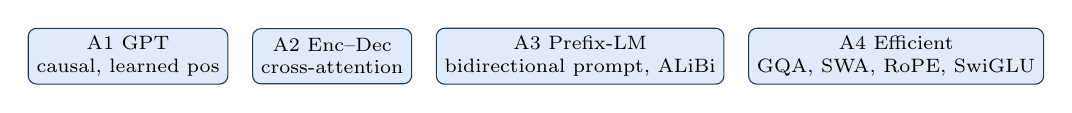
\begin{tikzpicture}[node distance=3mm]
        \node[hot] (a) {A1 GPT\\causal, learned pos};
        \node[hot,right=of a] (b) {A2 Enc--Dec\\cross-attention};
        \node[hot,right=of b] (c) {A3 Prefix-LM\\bidirectional prompt, ALiBi};
        \node[hot,right=of c] (d) {A4 Efficient\\GQA, SWA, RoPE, SwiGLU};
      \end{tikzpicture}
      \end{center}
    \item One interface, one trainer, one decoder and one local evaluator make every experiment a single command, with its evidence saved automatically.
    \item The next steps are to run all four at full budget, choose decoding on the dev set, submit at least four distinct runs, and carry the best models into Phase 2.
  \end{itemize}
\end{frame}

\begin{frame}{References}
  \scriptsize
  \begin{itemize}
    \item Joshi et al. (2024). IL-TUR: Benchmark for Indian Legal Text Understanding and Reasoning. arXiv:2407.05399.
    \item Vaswani et al. (2017). Attention Is All You Need.
    \item Radford et al. (2019). Language Models are Unsupervised Multitask Learners (GPT-2).
    \item Raffel et al. (2020). Exploring the Limits of Transfer Learning with a Unified Text-to-Text Transformer (T5).
    \item Dong et al. (2019). Unified Language Model Pre-training (UniLM). Du et al. (2022). GLM.
    \item Press, Smith and Lewis (2022). Train Short, Test Long: Attention with Linear Biases (ALiBi).
    \item Su et al. (2021). RoFormer: Rotary Position Embedding.
    \item Touvron et al. (2023). LLaMA. Jiang et al. (2023). Mistral 7B. Gemma Team (2024). Gemma 2.
    \item Ainslie et al. (2023). GQA: Training Generalized Multi-Query Transformer Models.
    \item Shazeer (2020). GLU Variants Improve Transformer. Zhang and Sennrich (2019). RMSNorm.
    \item Sennrich, Haddow and Birch (2016). Neural Machine Translation of Rare Words with Subword Units (BPE).
    \item Holtzman et al. (2020). The Curious Case of Neural Text Degeneration (top-$p$).
    \item Zhang et al. (2020). BERTScore. Lin (2004). ROUGE. Papineni et al. (2002). BLEU.
    \item Hinton, Vinyals and Dean (2015). Distilling the Knowledge in a Neural Network.
    \item Karpathy. nanoGPT (training-loop and token-bin design).
  \end{itemize}
\end{frame}

\end{document}
